\documentclass[11pt,onecolumn]{IEEEtran}
\usepackage{amsmath,amssymb,amsthm}
\usepackage{graphicx}
\usepackage[hidelinks]{hyperref}

\newtheorem{theorem}{Theorem}
\newtheorem{proposition}[theorem]{Proposition}
\newtheorem{corollary}[theorem]{Corollary}
\newtheorem{lemma}[theorem]{Lemma}
\newtheorem{conjecture}[theorem]{Conjecture}
\newtheorem{remark}[theorem]{Remark}

\newcommand{\E}{\mathbb{E}}
\newcommand{\R}{\mathbb{R}}
\newcommand{\C}{\mathbb{C}}
\newcommand{\tr}{\operatorname{tr}}
\newcommand{\Cov}{\operatorname{Cov}}
\newcommand{\Var}{\operatorname{Var}}
\newcommand{\hY}{\hat{\mathbf Y}}
\newcommand{\Sez}{\Sigma_{e0}}
\newcommand{\tQ}{\tilde Q}
\newcommand{\tH}{\tilde H}
\newcommand{\dw}{\tfrac{d\omega}{2\pi}}
\newcommand{\herm}{\mathsf H}

\emergencystretch=1.5em
\begin{document}

\title{Rate, Leakage, and Distortion for Stationary Gaussian Sources:\\ Water-Filling on a Tilted Spectrum}

\author{Andrew~H.~Bond,~\IEEEmembership{Senior Member,~IEEE}%
\thanks{A. H. Bond is with the Department of Computer Engineering, San Jos\'e
State University, San Jos\'e, CA 95192 USA (e-mail: andrew.bond@sjsu.edu).
The manuscript sources, the check scripts, and the notebook of
Appendix~\ref{app:numver} are in the public repository named there.}}

\markboth{Draft, November 2026}{Bond: Rate, Leakage, and Distortion for Stationary Gaussian Sources}

\maketitle

\begin{abstract}
An encoder describes part of a stationary Gaussian vector process to a
decoder under a weighted quadratic distortion. A second party holds a
noisy filtered observation of the process and never decodes. The
description has two costs per symbol, its rate and its conditional
leakage to the second party. For memoryless sources the frontier is
reverse water-filling on the decoder's weight tilted by the second
party's information. We show that for sources with memory the same
statement holds frequency by frequency, with one water level shared by
all frequencies. For a source with a finite period the region splits
exactly over the discrete Fourier frequencies, and as the period grows
it converges to a spectral region. Kolmogorov's reverse water-filling is the case of no
second party. For a scalar process with a scalar context the minimum
leakage is an integral of a closed form, and the two optimal
descriptions can occupy disjoint frequency bands. A delay in the second
party's observation changes nothing when that party keeps its whole
observation. When it keeps one sample or a causal prefix, the leakage
of a one-symbol description depends on what is kept through a single
conditional variance. For the stationary source itself we prove a
converse through finite windows. When the spectral density matrix is
affine in one scalar spectrum, the windows converge to the spectral
region and we prove a matching coding theorem, so the spectral region
is the operational region of the stationary source.
\end{abstract}

\begin{IEEEkeywords}
Equivocation, Gaussian processes, information leakage, rate--distortion
theory, secure source coding, spectral density, Toeplitz matrices,
water-filling.
\end{IEEEkeywords}

\section{Introduction}
\label{sec:intro}

A description of a signal is often held by more than one party. The
decoder that reconstructs from it pays its rate. A second party that
holds the description together with its own observation of the source
learns from it the conditional mutual information between the source and
the description given that observation. In a secrecy reading this is
the leakage to an eavesdropper with side information. In a storage
reading it is the least rate at which the second party can keep the
description compressed against what it already holds. The companion
paper \cite{part1} determines how the two costs trade off for a
memoryless Gaussian vector source. Its main statement is that each
frontier point is the fixed point of reverse water-filling on the
decoder's weight tilted by the information the second party's
observation adds to the description \cite[Theorem~7]{part1}.

Signals have memory, and the second party's observation of a signal is
usually filtered, delayed, or incomplete. This paper treats a stationary
Gaussian vector process $T_t$ with spectral density matrix
$\Sigma(\omega)$. The decoder reproduces $Y_t=FT_t$ under a weighted
quadratic distortion per symbol. The second party, called the holder as
in \cite{part1}, observes a filtered copy of the process in stationary
Gaussian noise. The costs are the rate and the leakage per symbol.

The results are as follows. For a source of period $n$, by which we
mean independent blocks of length $n$ with a block-circulant
covariance, the frontier splits exactly over the $n$ discrete Fourier
frequencies. At each frequency the error spectrum solves the tilted
water-filling equation of \cite{part1} for Hermitian data, and one water
level is common to all frequencies (Theorem~\ref{thm:periodic}). As $n$
grows, the frontier converges to a spectral program whose solution is
the same equation at every frequency under one level
(Theorem~\ref{thm:spectral}). With no holder this is reverse
water-filling for Gaussian processes \cite{kolmogorov1956,berger1971}.
With a holder, the level is shared but the weight being filled is
tilted differently at each frequency, by an amount that depends on the
solution there.

For a scalar process with a scalar context and a holder that observes
the context in noise, the minimum leakage is the integral over
frequency of the scalar closed form of \cite[Corollary~17]{part1},
under a distortion allocation that equalizes slopes
(Theorem~\ref{thm:pair}). The rate-optimal description describes the
frequencies where the spectrum of $Y$ is largest. The leakage-optimal
description describes the frequencies where that spectrum times a
factor set by the coherence with the context and the holder's noise is
largest. The two orders can disagree completely, and then the two
descriptions occupy disjoint bands (Corollary~\ref{cor:bands}). This is
the allocation among independent components of
\cite[Theorem~27]{part1} with frequencies as the components. The
mechanism is inherited. What a signal adds is that the components need
not be supplied by the model, since stationarity supplies them.

The holder's filter enters every result only through
$J(\omega)=H(\omega)^{\herm}\Sigma_U(\omega)^{-1}H(\omega)$. A delay, or
any all-pass filter, therefore changes nothing
(Proposition~\ref{prop:allpass}). This holds because the holder keeps
its whole observation. Section~\ref{sec:retention} asks what happens
when it keeps less. For a description of one symbol, the leakage
depends on what the holder keeps only through the conditional variance
of the context given what is kept (Proposition~\ref{prop:retention}).
For a first-order autoregressive context this gives the leakage in
closed form when the holder keeps one sample at lag $\Delta$, and a
geometric interpolation in $\Delta$ between the filtering and the
smoothing values when it keeps a causal prefix. So a delay costs
nothing to a party that holds its whole observation when it uses it,
and the cost of a stale observation is the cost of holding less: fewer
samples kept, or samples that have not yet arrived.

The period-$n$ source is a model. For the stationary source itself we
prove that every code of blocklength $N$ lies in the region of the
$N$-symbol window (Proposition~\ref{prop:window}). When the spectral
density matrix is affine in one scalar spectrum, which covers a
process observed through memoryless maps in white noise, the window
problem splits exactly in the eigenbasis of a Toeplitz matrix at every
$N$, and the window regions converge to the spectral region by
Szeg\H{o}'s theorem (Theorem~\ref{thm:affine}). For general spectra
the convergence of the windows is a conjecture, supported by
computation (Conjecture~\ref{conj:windows}).

For the affine class we also prove achievability for the stationary
source, so there the spectral region is the operational region
(Theorem~\ref{thm:achieve}). The proof writes the source as a
finite-memory source plus an independent source of small power. Blocks
of a finite-memory source separated by guard intervals are independent,
so the memoryless theorem of \cite{part1} codes them. The encoder sees
only the sum and draws the finite-memory part from its conditional law,
which makes the encoder randomized, and the small remainder changes the
leakage by an amount that vanishes with its power. For a general
spectrum the same argument reduces achievability to the convergence of
the windows.

\subsection*{Related work}

The single-letter region of rate, distortion, and equivocation is due
to Villard and Piantanida \cite{villard2013}. Ekrem and Ulukus
\cite{ekrem2013} and Xu, Chen, Chen, and Jin \cite{xu2024} treat
memoryless vector Gaussian sources under a matrix distortion. The
structure of the region under a trace-type distortion, for memoryless
sources, is the subject of \cite{part1}, on which every proof here
rests. We found no rate--distortion--equivocation result for a Gaussian
source with memory and side information at the second party. The
closest results are these. Sankar, Rajagopalan, Mohajer, and Poor
\cite{sankar2011,sankar2013} study the tradeoff between utility and
privacy for a scalar stationary Gaussian source whose private part is a
noisy scaling of the source, and obtain spectral allocations by
filtering frequency components. Their leakage is the unconditional
mutual information between the private sequence and the
reconstruction, and the adversary has no side information. Here the
leakage is conditional on a second party's own observation of the
source, and that observation is what tilts the weight at each
frequency.
% verify on final: this comparison was written from the conference version (arXiv:1108.2234 = SmartGridComm 2011).
% The T-SG 2013 journal text has NOT been read. A reviewer of this draft reports that the journal version states that
% rate and leakage cannot in general be minimised together and develops an interference-aware spectral allocation.
% An earlier draft of this paragraph said their rate-optimal solution is also leakage-optimal; that sentence was removed
% until the journal text is read and the assumptions can be stated exactly. Liu,
Cuff, and Verd\'u \cite{liu2016} obtain the key capacity of jointly
stationary Gaussian processes by treating frequencies as a product
source with one water level. Their problem is key agreement and has no
distortion. Dikshtein, Weinberger, and Shamai \cite{dikshtein2022}
solve the information bottleneck for Gaussian processes by spectral
water-filling and define, without solving, the privacy funnel for
them. Conditional rate--distortion theory for sources with memory goes
back to Gray \cite{gray1973} and Leiner and Gray \cite{leiner1974}, and
spectral formulas for remote sources to Dobrushin and Tsybakov
\cite{dobrushin1962}. Simeone and Permuter \cite{simeone2013} show that
delayed side information at a decoder changes the rate when the
decoder is causally constrained. Proposition~\ref{prop:allpass} is the
complementary statement for a party that is not constrained.

The technique is standard. Splitting a circulant problem over Fourier
frequencies and passing to the spectral limit is the classical route
to rate--distortion functions of Gaussian processes
\cite{berger1971,pearl1973,gray2006}, and the eigenvalue distribution
of Toeplitz matrices is Szeg\H{o}'s theorem
\cite{grenander1958,gray2006}. What is new is the object to which it is
applied, a two-cost program whose per-frequency solution is not a
function of the spectrum alone.

\section{Model}
\label{sec:model}

Logarithms are base two unless written $\ln$. Notation follows
\cite{part1}. For a Hermitian matrix $A\succeq0$ with eigenpairs
$(\lambda_i,e_i)$,
$\Phi(A)=\sum_i\min\{1,1/\lambda_i\}e_ie_i^{\herm}$, with
$\min\{1,1/\lambda_i\}=1$ when $\lambda_i=0$.

\subsection{The stationary source}

Let $(T_t)_{t\in\mathbb Z}$ be a centered stationary Gaussian process in
$\R^p$ with autocovariance $R(\tau)=\E[T_{t+\tau}T_t^{\mathsf T}]$ and
spectral density matrix
$\Sigma(\omega)=\sum_\tau R(\tau)e^{-i\omega\tau}$. We assume $\Sigma$ is
continuous on $[-\pi,\pi]$ with $\Sigma(\omega)\succ0$ for every
$\omega$. The described process is $Y_t=FT_t\in\R^m$ with $F$ of full row
rank, the decoder's weight is $W\succ0$, and $Q=F^{\mathsf T}WF$. The
holder observes
\[
S_t=\sum_k H_kT_{t-k}+U_t\in\R^r ,
\]
where $(U_t)$ is a centered stationary Gaussian process independent of
$(T_t)$ with continuous spectral density $\Sigma_U(\omega)\succ0$, and the
filter has a continuous frequency response
$H(\omega)=\sum_kH_ke^{-i\omega k}$. Write
\[
J(\omega)=H(\omega)^{\herm}\Sigma_U(\omega)^{-1}H(\omega),\qquad
D_{\max}=\int_{-\pi}^{\pi}\tr\bigl(Q\Sigma(\omega)\bigr)\dw .
\]

\subsection{The source of period $n$}

Let $\omega_k=2\pi k/n$ for $k=0,\dots,n-1$, and let
$\mathsf U_n$ be the unitary matrix with blocks
$n^{-1/2}e^{i\omega_ka}I$ in block row $a$ and block column $k$. The
source of period $n$ emits independent copies of a block
$T^{(n)}=(T_0,\dots,T_{n-1})\in\R^{pn}$ with covariance
\[
\Sigma_n=\mathsf U_n\operatorname{diag}\bigl(\Sigma(\omega_0),\dots,\Sigma(\omega_{n-1})\bigr)\mathsf U_n^{\herm},
\]
the block-circulant matrix whose block $(a,b)$ is
$\tfrac1n\sum_k\Sigma(\omega_k)e^{i\omega_k(a-b)}$. It is real because
$\Sigma(-\omega)=\overline{\Sigma(\omega)}$. The holder observes
$S^{(n)}=H_nT^{(n)}+U^{(n)}$, where $H_n$ and $\Cov U^{(n)}$ are the
block-circulant matrices with symbols $H$ and $\Sigma_U$. This is the
stationary source with time wrapped around a circle of $n$ symbols. Its
blocks are independent, so it is a memoryless source with letters in
$\R^{pn}$, and \cite[Theorem~3]{part1} applies to it with weight
$Q_n=\tfrac1nI_n\otimes Q$. We measure rate, leakage, and distortion per
symbol, that is, per block divided by $n$.

\subsection{Per-frequency costs}

For a Hermitian $p\times p$ matrix $X$ with $0\prec X\preceq I$ and a
frequency $\omega$, let
\begin{align*}
\tQ(\omega)&=\Sigma(\omega)^{1/2}Q\,\Sigma(\omega)^{1/2},&
\tH(\omega)&=H(\omega)\Sigma(\omega)^{1/2},\\
r(X)&=-\tfrac12\log\det X,&
d_\omega(X)&=\tr\bigl(\tQ(\omega)X\bigr),
\end{align*}
\begin{equation}
\ell_\omega(X)=r(X)-\tfrac12\log\frac{\det\bigl(\tH\tH^{\herm}+\Sigma_U\bigr)}{\det\bigl(\tH X\tH^{\herm}+\Sigma_U\bigr)}
=\tfrac12\log\frac{\det\bigl(X^{-1}+\tilde J\bigr)}{\det\bigl(I+\tilde J\bigr)},
\label{eq:ell}
\end{equation}
with $\tH$ and $\Sigma_U$ evaluated at $\omega$ and
$\tilde J=\Sigma^{1/2}J\Sigma^{1/2}$. The matrix
$\Sigma(\omega)^{1/2}X\Sigma(\omega)^{1/2}$ is the spectral density of the
error in estimating $T$ from the description, and $X$ is that error
spectrum in whitened coordinates. The two forms of $\ell_\omega$ agree by
the determinant identity of \cite[eq.~(11)]{part1}. For
$\alpha\in[0,1]$ write
$f_{\alpha,\omega}=\alpha r+(1-\alpha)\ell_\omega$ and
\begin{equation}
\mathcal T_{\alpha,\omega}(X)=(1-\alpha)\,\tH^{\herm}\bigl(\tH X\tH^{\herm}+\Sigma_U\bigr)^{-1}\tH ,
\label{eq:tilt}
\end{equation}
the tilt. It equals $(1-\alpha)X^{-1}\bigl(X-(X^{-1}+\tilde J)^{-1}\bigr)X^{-1}$,
so it depends on the holder only through $J(\omega)$.

\section{Hermitian Data and One Compactness Lemma}
\label{sec:tools}

The results of \cite{part1} are stated for real symmetric matrices. The
frequency blocks are Hermitian. The next lemma transfers what we need.

\begin{lemma}\label{lem:hermitian}
Let $\tQ\succeq0$ be Hermitian $p\times p$, $\tH\in\C^{r\times p}$, and
$\Sigma_U\succ0$ Hermitian, and define $r$, $\ell$, $d$, $f_\alpha$, and
$\mathcal T_\alpha$ from them as in Section~\ref{sec:model}. For
$\alpha\in[0,1]$ and $\nu>0$ the function
$f_\alpha(X)\ln2+\nu\,d(X)$ has a unique minimizer $X(\nu)$ over Hermitian
$0\prec X\preceq I$. It is the unique solution of
\begin{equation}
X=\Phi\bigl(2\nu\tQ+\mathcal T_\alpha(X)\bigr),
\label{eq:fixed}
\end{equation}
and $X(\nu)\succeq\min\{1,1/\Lambda\}I$ with
$\Lambda=\lambda_{\max}(2\nu\tQ+\tH^{\herm}\Sigma_U^{-1}\tH)$. Both $r$ and
$\ell$ are strictly convex on $\{0\prec X\preceq I\}$. The distortion
$d(X(\nu))$ is nonincreasing in $\nu$ and at most $p/\nu$. If the data
are real, $X(\nu)$ is real.
\end{lemma}

\begin{proof}
For a complex matrix $A=A_1+iA_2$ let
$\varrho(A)=\bigl[\begin{smallmatrix}A_1&-A_2\\A_2&A_1\end{smallmatrix}\bigr]$.
The map $\varrho$ is real-linear, multiplicative, and takes adjoints to
transposes, so it takes Hermitian matrices to real symmetric ones and
preserves the L\"owner order. Each eigenvalue of a Hermitian $A$ is an
eigenvalue of $\varrho(A)$ with twice the multiplicity, so
$\det\varrho(A)=(\det A)^2$, $\tr\varrho(A)=2\tr A$, and
$\Phi(\varrho(A))=\varrho(\Phi(A))$. Consider the real problem of
\cite{part1} in whitened coordinates with data $\varrho(\tQ)$,
$\varrho(\tH)$, $\varrho(\Sigma_U)$ and dimension $2p$. On matrices of the
form $\varrho(X)$ its rate, leakage, and distortion are twice $r(X)$,
$\ell(X)$, and $d(X)$. By \cite[Theorem~5]{part1} its rate and leakage
are strictly convex, and by the proof of \cite[Theorem~7]{part1} and
\cite[Remark~10]{part1} the penalized objective has a unique minimizer
$\mathsf X$ over real symmetric $0\prec\mathsf X\preceq I$, which is the
unique solution of the real form of \eqref{eq:fixed}. Let
$\mathsf J=\bigl[\begin{smallmatrix}0&-I\\I&0\end{smallmatrix}\bigr]$. It is
orthogonal and commutes with every $\varrho(A)$, so
$\mathsf X\mapsto\mathsf J\mathsf X\mathsf J^{\mathsf T}$ preserves the
penalized objective and the constraint set. By uniqueness
$\mathsf J\mathsf X=\mathsf X\mathsf J$, and a real symmetric matrix that
commutes with $\mathsf J$ is $\varrho(X)$ for a Hermitian $X$. So the
minimizer of the real problem lies in the image of $\varrho$, and its
preimage $X(\nu)$ is the unique minimizer of the Hermitian problem and
the unique Hermitian solution of \eqref{eq:fixed}. Strict convexity
restricts to the image of $\varrho$. The lower bound is the one in the
proof of \cite[Proposition~11]{part1}: every eigenvalue of
$2\nu\tQ+\mathcal T_\alpha(X)$ is at most $\Lambda$ because
$\mathcal T_\alpha(X)\preceq\tH^{\herm}\Sigma_U^{-1}\tH$, and $\Phi$ maps an
eigenvalue $\lambda$ to $\min\{1,1/\lambda\}$. The same proof gives
$d(\Phi(2\nu\tQ+\mathcal T))\le\sum_i2q_i/(2\nu q_i+1)\le p/\nu$ for every
$\mathcal T\succeq0$, with $q_i$ the eigenvalues of $\tQ$. Monotonicity
in $\nu$ is the comparison of the penalized minima at two levels. If
the data are real, entrywise conjugation preserves the objective and
the constraints, so the unique minimizer is real.
\end{proof}

The two limits in this paper, over Fourier frequencies and over Toeplitz
eigenvalues, are instances of one statement.

\begin{lemma}\label{lem:limit}
Let $K$ be a compact metric space and let
$u\mapsto(\tQ(u),\tH(u),\Sigma_U(u))$ be continuous on $K$, with
$\Sigma_U(u)\succ0$. Write $X(u,\nu)$ for the minimizer of
Lemma~\ref{lem:hermitian} at $u$, with $X(u,0)=I$, and
$d(u,\nu)=\tr(\tQ(u)X(u,\nu))$. Let $\mu_n$ be Borel probability
measures on $K$ that converge weakly to $\mu$, and let
$0<D<\int\tr\tQ\,d\mu$. For a probability measure $\lambda$ on $K$ let
\[
V_\lambda(\alpha,D)=\inf\Bigl\{\int f_{\alpha,u}\bigl(X(u)\bigr)\,d\lambda(u):\
\int\tr\bigl(\tQ(u)X(u)\bigr)\,d\lambda(u)\le D\Bigr\},
\]
the infimum over measurable Hermitian fields with $0\prec X(u)\preceq I$.
\begin{enumerate}
\item[(a)] $X(u,\nu)$ is jointly continuous on $K\times[0,\infty)$.
\item[(b)] For $\lambda=\mu$ and for $\lambda=\mu_n$ with $n$ large, there
is a level $\nu_\lambda\in(0,p/D]$ with $\int d(u,\nu_\lambda)\,d\lambda=D$.
For every such level the field $X(\cdot,\nu_\lambda)$ attains
$V_\lambda(\alpha,D)$, and every minimizer equals it
$\lambda$-almost everywhere.
\item[(c)] $V_{\mu_n}(\alpha,D)\to V_\mu(\alpha,D)$, and the rate
$\int r(X(u,\nu_{\mu_n}))\,d\mu_n$ and leakage
$\int\ell_u(X(u,\nu_{\mu_n}))\,d\mu_n$ of the minimizers converge to those
of the minimizer for $\mu$.
\end{enumerate}
\end{lemma}

\begin{proof}
(a) Fix $\bar\nu>0$. The eigenvalue bound of Lemma~\ref{lem:hermitian} is
uniform over $K\times[0,\bar\nu]$ by compactness, so there is $\delta>0$
with $X(u,\nu)\in\mathcal K_\delta=\{\delta I\preceq X\preceq I\}$ on that
set. The penalized objective is jointly continuous on
$K\times[0,\bar\nu]\times\mathcal K_\delta$ and has a unique minimizer
over the compact set $\mathcal K_\delta$ for each $(u,\nu)$. If
$(u_j,\nu_j)\to(u,\nu)$ and a subsequence of $X(u_j,\nu_j)$ converges to
$\bar X$, passing to the limit in the inequalities that say
$X(u_j,\nu_j)$ is a minimizer shows that $\bar X$ minimizes at $(u,\nu)$,
so $\bar X=X(u,\nu)$. This is Berge's maximum theorem
\cite[Ch.~VI, \S3]{berge1963} for a single-valued minimizer.

(b) The map $\nu\mapsto\int d(u,\nu)\,d\lambda$ is continuous by (a) and
bounded convergence, equals $\int\tr\tQ\,d\lambda$ at $\nu=0$, which
exceeds $D$ for $\lambda=\mu$ and for $\lambda=\mu_n$ with $n$ large by
weak convergence, and is at most $p/\nu$. So a level $\nu_\lambda$
exists, and $\nu_\lambda\le p/D$. For any feasible field,
\[
\int f_{\alpha,u}(X(u))\ln2\,d\lambda\ \ge\ \int\bigl[f_{\alpha,u}(X(u))\ln2+\nu_\lambda\tr(\tQ X(u))\bigr]d\lambda-\nu_\lambda D
\ \ge\ \int f_{\alpha,u}\bigl(X(u,\nu_\lambda)\bigr)\ln2\,d\lambda ,
\]
the second step by pointwise minimality and
$\int d(u,\nu_\lambda)\,d\lambda=D$. Equality in the second step forces
$X(u)=X(u,\nu_\lambda)$ almost everywhere, by uniqueness of the pointwise
minimizer.

(c) On $K\times[0,p/D]$ the functions $d$,
$r(X(u,\nu))$, and $\ell_u(X(u,\nu))$ are continuous, hence uniformly
continuous, so for each of them the family indexed by $\nu$ is a
compact subset of $C(K)$, and weak convergence is uniform on compact
subsets of $C(K)$. Let $\nu^\ast$ be a limit point of $\nu_{\mu_n}$. Then
$\int d(u,\nu^\ast)\,d\mu=\lim\int d(u,\nu_{\mu_n})\,d\mu_n=D$, so
$X(\cdot,\nu^\ast)$ is the minimizer for $\mu$ by (b), and the rate and
leakage integrals converge along the subsequence to its rate and
leakage. The minimizer for $\mu$ is unique almost everywhere, so every
limit point gives the same limits.
\end{proof}

The second inequality in the proof of (b) is the statement that an
allocation with a common slope is optimal. It and its finite form are
machine-checked (Appendix~\ref{app:numver}).

\section{The Source of Period $n$}
\label{sec:periodic}

\begin{theorem}\label{thm:periodic}
Let $\alpha\in[0,1]$ and
$0<D<\tfrac1n\sum_k\tr(Q\Sigma(\omega_k))$. The frontier point of weight
$\alpha$ of the source of period $n$ is, in the whitened coordinate of
\cite{part1},
\[
X_n=\mathsf U_n\operatorname{diag}(X_0,\dots,X_{n-1})\,\mathsf U_n^{\herm},
\]
where the Hermitian matrices $X_k$ are the solutions of
\begin{equation}
X_k=\Phi\Bigl(2\nu\,\tQ(\omega_k)+\mathcal T_{\alpha,\omega_k}(X_k)\Bigr),
\qquad
\frac1n\sum_{k=0}^{n-1}d_{\omega_k}(X_k)=D ,
\label{eq:periodic}
\end{equation}
for one level $\nu>0$, and $X_{n-k}=\overline{X_k}$. Its rate and
leakage per symbol are $\tfrac1n\sum_kr(X_k)$ and
$\tfrac1n\sum_k\ell_{\omega_k}(X_k)$. The weighted cost
$\tfrac1n\sum_kf_{\alpha,\omega_k}(X_k)$ is the minimum of
$\tfrac1n\sum_kf_{\alpha,\omega_k}(Z_k)$ over Hermitian
$0\prec Z_k\preceq I$ with $\tfrac1n\sum_kd_{\omega_k}(Z_k)\le D$.
\end{theorem}

\begin{proof}
Let $P$ be the cyclic shift on $\R^n$ and $\mathsf P_p=P\otimes I_p$, a real
orthogonal matrix. A matrix commutes with $\mathsf P_p$ if and only if it
is block-circulant, and the block-circulant matrices are those of the
form $\mathsf U_n\operatorname{diag}(A_k)\mathsf U_n^{\herm}$. So
$\Sigma_n^{1/2}=\mathsf U_n\operatorname{diag}(\Sigma(\omega_k)^{1/2})\mathsf U_n^{\herm}$
commutes with $\mathsf P_p$, as does
$\tQ_n=\Sigma_n^{1/2}Q_n\Sigma_n^{1/2}=\mathsf U_n\operatorname{diag}(\tfrac1n\tQ(\omega_k))\mathsf U_n^{\herm}$,
while $\tH_n=H_n\Sigma_n^{1/2}$ satisfies $\tH_n\mathsf P_p=\mathsf P_r\tH_n$
and $\Cov U^{(n)}$ commutes with $\mathsf P_r$. The map
$X\mapsto\mathsf P_pX\mathsf P_p^{\mathsf T}$ therefore preserves
$\det X$, the distortion $\tr(\tQ_nX)$, the constraint
$0\prec X\preceq I$, and
$\det(\tH_nX\tH_n^{\mathsf T}+\Cov U^{(n)})$, which becomes the
determinant of the same matrix conjugated by $\mathsf P_r$. By
\cite[Theorem~5(a)]{part1} the frontier point $X_n$ is the unique
minimizer of the weighted program, so
$\mathsf P_pX_n\mathsf P_p^{\mathsf T}=X_n$. Hence $X_n$ is block-circulant,
$X_n=\mathsf U_n\operatorname{diag}(X_k)\mathsf U_n^{\herm}$ with $X_k$
Hermitian, and $X_{n-k}=\overline{X_k}$ because $X_n$ is real. By
\cite[Theorem~7]{part1},
$X_n=\Phi(2\nu_n\tQ_n+\mathcal T_n(X_n))$ for some $\nu_n>0$, with
$\mathcal T_n$ the tilt of the block problem, and
$\tr(\tQ_nX_n)=D$. Conjugation by $\mathsf U_n$ turns
$2\nu_n\tQ_n+\mathcal T_n(X_n)$ into the block-diagonal matrix with blocks
$2(\nu_n/n)\tQ(\omega_k)+\mathcal T_{\alpha,\omega_k}(X_k)$, and $\Phi$ is a
spectral function, so it commutes with unitary conjugation and acts
block by block. This is \eqref{eq:periodic} with $\nu=\nu_n/n$. The
determinants in the two costs are products over $k$, which gives the
rate and leakage. For the last statement, the fields $(Z_k)$ and the
measure $\tfrac1n\sum_k\delta_{\omega_k}$ are an instance of
Lemma~\ref{lem:limit}(b), whose minimizer is the solution of
\eqref{eq:periodic}.
\end{proof}

The frequencies are coupled only through the one level $\nu$. The tilt
at frequency $\omega_k$ depends on the solution at that frequency and on
no other. In \cite{part1} the region splits along subspaces that the
decoder's and the holder's geometries share
\cite[Theorem~12]{part1}. Stationarity supplies such subspaces for every
source, the Fourier frequencies, whatever the two geometries are within
each frequency.

\section{The Spectral Region}
\label{sec:spectral}

Let $V_n(\alpha,D)$ be the weighted cost per symbol of the frontier
point of Theorem~\ref{thm:periodic}, and $(R_n,L_n)$ its rate and
leakage.

\begin{theorem}\label{thm:spectral}
Let $\alpha\in[0,1]$ and $0<D<D_{\max}$. As $n\to\infty$,
$V_n(\alpha,D)\to V(\alpha,D)$ and $(R_n,L_n)\to(R,L)$, where
\begin{equation}
V(\alpha,D)=\min\Bigl\{\int_{-\pi}^{\pi}f_{\alpha,\omega}\bigl(X(\omega)\bigr)\dw:\
\int_{-\pi}^{\pi}\tr\bigl(\tQ(\omega)X(\omega)\bigr)\dw\le D\Bigr\}
\label{eq:spectralprogram}
\end{equation}
over measurable Hermitian fields $0\prec X(\omega)\preceq I$. The minimum
is attained, uniquely up to a null set, by the continuous field that
solves
\begin{equation}
X(\omega)=\Phi\Bigl(2\nu\,\tQ(\omega)+(1-\alpha)\,\tH(\omega)^{\herm}\bigl(\tH(\omega)X(\omega)\tH(\omega)^{\herm}+\Sigma_U(\omega)\bigr)^{-1}\tH(\omega)\Bigr)
\label{eq:spectral}
\end{equation}
at every frequency, for one level $\nu>0$ at which the distortion
constraint holds with equality, and
\[
R=\int_{-\pi}^{\pi}r\bigl(X(\omega)\bigr)\dw,\qquad
L=\int_{-\pi}^{\pi}\ell_\omega\bigl(X(\omega)\bigr)\dw .
\]
\end{theorem}

\begin{proof}
Apply Lemma~\ref{lem:limit} with $K$ the circle, the data of
Section~\ref{sec:model}, which are continuous because $\Sigma^{1/2}$ is,
$\mu_n$ the uniform measure on $\{\omega_k\}$, and $\mu$ the normalized
Lebesgue measure. By Theorem~\ref{thm:periodic},
$V_n(\alpha,D)=V_{\mu_n}(\alpha,D)$.
\end{proof}

The spectral region at distortion $D$ is
\begin{equation}
\mathcal R(D)=\bigl\{(R,L):\ \alpha R+(1-\alpha)L\ge V(\alpha,D)\ \text{ for every }\alpha\in[0,1]\bigr\},
\label{eq:region}
\end{equation}
a closed, convex, upward closed set. The frontier point of weight
$\alpha$ lies on its boundary, since it meets the bound of weight $\alpha$
with equality and satisfies the others because its field is feasible
for every weight. Write $R_{\min}(D)=V(1,D)$ and $L(D)=V(0,D)$ for the
least rate and least leakage. At $\alpha=1$ the tilt vanishes
and \eqref{eq:spectral} is reverse water-filling of the spectrum of
$\tQ(\omega)$ at the common level $1/(2\nu)$. For a scalar described
process this is Kolmogorov's formula
\cite{kolmogorov1956,berger1971}: with
$S_Y(\omega)=\tr(Q\Sigma(\omega))$ and $\theta=1/(2\nu)$,
\[
R_{\min}(D)=\int_{-\pi}^{\pi}\max\Bigl\{0,\tfrac12\log\frac{S_Y(\omega)}{\theta}\Bigr\}\dw,
\qquad
D=\int_{-\pi}^{\pi}\min\{\theta,S_Y(\omega)\}\dw .
\]
For $\alpha<1$ the level is still common, but the matrix being filled
at frequency $\omega$ is the decoder's weight plus the information the
holder's observation adds to the description at that frequency. By
\cite[Corollary~8]{part1} applied at each frequency, the frontier
description is the rate--distortion optimal description for a decoder
that must also reproduce the holder's noiseless view $H\ast T$, under a
frequency-dependent weight fixed by the solution.

When $\tQ(\omega)$ and $\tilde J(\omega)$ commute at every frequency, the
solution is explicit. In a common eigenbasis with eigenvalues
$q_i(\omega)$ and $j_i(\omega)$, \cite[Theorem~13]{part1} gives the
error spectrum as follows. A direction with $q_i(\omega)=0$ does not
enter the distortion and has $x_i(\omega)=1$. This case occurs because
$Q=F^{\mathsf T}WF$ may be rank deficient. Where $q_i(\omega)>0$,
$x_i(\omega)=\min\{1,\xi_i(\omega)\}$ with $\xi_i$ the positive root of
$\theta q_ij_ix^2+(\theta q_i-\alpha j_i)x-1=0$ and $\theta=2\nu$
($\xi_i=1/(\theta q_i)$ when $j_i=0$), and the direction is described at
that frequency exactly when
$\theta>(1+\alpha j_i(\omega))/(q_i(\omega)(1+j_i(\omega)))$.

\section{A Scalar Process with a Scalar Context}
\label{sec:pair}

Let $T_t=(Y_t,V_t)$ with spectra $S_Y$, $S_V$, cross-spectrum $S_{YV}$,
and coherence
$\kappa(\omega)=|S_{YV}(\omega)|^2/(S_Y(\omega)S_V(\omega))<1$. The decoder
reproduces $Y$ under squared error, and the holder observes
$S_t=(h\ast V)_t+U_t$ with $U$ of spectrum $S_U>0$. Write
\[
s(\omega)=1+\frac{S_U(\omega)}{|H(\omega)|^2S_V(\omega)}
\]
where $H(\omega)\ne0$. Let
$g^\star(\rho^2,s,\delta)$ be the larger root of
$\delta sg^2-(\delta+s-\rho^2)g+(1-\rho^2)$, the function of
\cite[Corollary~17]{part1}, and
\[
\ell(\omega,d)=\tfrac12\log g^\star\Bigl(\kappa(\omega),s(\omega),\frac{d}{S_Y(\omega)}\Bigr)
\quad\text{for }0<d<S_Y(\omega),\qquad
\ell(\omega,d)=0\quad\text{for }d\ge S_Y(\omega).
\]
Where $H(\omega)=0$ set $\ell(\omega,d)=\tfrac12\log(S_Y(\omega)/d)$, the
limit as $s\to\infty$.

\begin{theorem}\label{thm:pair}
For $0<D<D_{\max}=\int S_Y\,\dw$,
\[
L(D)=\min\Bigl\{\int_{-\pi}^{\pi}\ell\bigl(\omega,D(\omega)\bigr)\dw:\ \int_{-\pi}^{\pi}D(\omega)\dw\le D\Bigr\}.
\]
The minimizing allocation is unique and continuous. With
\begin{equation}
G(\omega)=S_Y(\omega)\Bigl(1+\frac{\kappa(\omega)|H(\omega)|^2S_V(\omega)}{S_U(\omega)}\Bigr),
\qquad
\vartheta_0(\omega)=\frac{1}{2\ln2\;G(\omega)},
\label{eq:G}
\end{equation}
it is $D(\omega)=S_Y(\omega)$ where $\vartheta\le\vartheta_0(\omega)$, and
elsewhere the solution of
$-\partial\ell(\omega,d)/\partial d=\vartheta$, for the level $\vartheta$
at which $\int D(\omega)\,\dw=D$. So the leakage-optimal description
describes the frequencies at which $G(\omega)$ exceeds
$1/(2\vartheta\ln2)$, while the rate-optimal description describes those
at which $S_Y(\omega)$ exceeds its water level. Where $H(\omega)\ne0$,
$G=S_Y(1+\kappa/(s-1))$, and where $H(\omega)=0$, $G=S_Y$.
\end{theorem}

\begin{proof}
At $\alpha=0$ the penalized minimum of Lemma~\ref{lem:hermitian} at
frequency $\omega$ is
$\min_d[\lambda(\omega,d)\ln2+\nu d]$, where $\lambda(\omega,d)$ is the
least value of $\ell_\omega(X)$ over $0\prec X\preceq I$ with
$d_\omega(X)\le d$. We show $\lambda=\ell$. The costs and the constraint
are unchanged when $T$ is replaced by $MT$ for an invertible complex
matrix $M$, with $F$ and $H$ replaced by $FM^{-1}$ and $HM^{-1}$, because
$X$ changes by a unitary similarity. Take
$M=\operatorname{diag}(S_Y^{-1/2},e^{i\phi}S_V^{-1/2})$ with $\phi$ the
phase of $S_{YV}$. The source then has unit variances and real
correlation $\sqrt{\kappa}$, the weight is $S_Ye_1e_1^{\mathsf T}$, and
after dividing the holder's observation by $H S_V^{1/2}e^{-i\phi}$ the
holder sees the second coordinate in noise of variance $s-1$. The data
are real, so by the conjugation argument of Lemma~\ref{lem:hermitian}
the minimizer is real and the problem is the real scalar problem of \cite[Corollary~17]{part1} at
normalized distortion $d/S_Y$, whose least leakage is $\ell(\omega,d)$.
By \cite[Lemma~26]{part1}, $\ell(\omega,\cdot)$ is strictly convex and
decreasing on $(0,S_Y)$, its slope tends to $-\infty$ at $0$ and to
$-(s-1)/(2\ln2\,S_Y(s-1+\kappa))=-\vartheta_0(\omega)$ at $S_Y$. Where
$H(\omega)=0$ the same holds for $\tfrac12\log(S_Y/d)$ with
$\vartheta_0=1/(2\ln2\,S_Y)$. So the minimizing $d$ is the stated one
with $\vartheta=\nu/\ln2$, and the claim is Theorem~\ref{thm:spectral} at
$\alpha=0$. Continuity of the allocation is Lemma~\ref{lem:limit}(a).
\end{proof}

The factor that reorders the frequencies is one plus the signal-to-noise
ratio of the part of the holder's observation that is coherent with
$Y$. A band in which the holder already sees much of what $Y$ contains
is cheap to describe in leakage, and the leakage-optimal description
starts there even if the band carries little of the power of $Y$.

\begin{corollary}\label{cor:bands}
Let $G$ be the function of \eqref{eq:G}. Suppose that
on $[0,\pi]$ the spectrum $S_Y$ attains its maximum only at $\omega_1$
and $G$ attains its maximum only at $\omega_2\ne\omega_1$. Then for every
$D$ close enough to $D_{\max}$ the rate-optimal and the leakage-optimal
descriptions describe disjoint sets of frequencies.
\end{corollary}

\begin{proof}
The rate-optimal description describes $\{S_Y>\theta\}$ with
$D=\int\min\{\theta,S_Y\}\,\dw$, so $\theta\to\max S_Y$ as $D\to D_{\max}$.
By Theorem~\ref{thm:pair} the leakage-optimal description describes
$\{G>c\}$ with $c=1/(2\vartheta\ln2)$. If $c$ stayed below
$\max G-\epsilon$ along a sequence $D\to D_{\max}$, the allocation would
lie strictly below $S_Y$ on the set $\{G>\max G-\epsilon\}$, which has
positive measure, by an amount bounded away from zero on a smaller set
of positive measure, since the allocation is continuous in the level.
That contradicts $\int D(\omega)\,\dw\to D_{\max}$. So $c\to\max G$. Both
functions are continuous and even, so the two sets shrink to
$\{\pm\omega_1\}$ and $\{\pm\omega_2\}$ and are eventually disjoint.
\end{proof}

Section~\ref{sec:examples} gives an instance and the range of budgets
over which its two descriptions are disjoint.

\section{Filters, Delay, and What the Holder Keeps}
\label{sec:retention}

\begin{proposition}\label{prop:allpass}
The period-$n$ region for every $n$, and the spectral region, depend on
the holder's filter and noise only through $J(\omega)$. In particular
they are unchanged when $H(\omega)$ is replaced by $A(\omega)H(\omega)$
and $\Sigma_U(\omega)$ by $A(\omega)\Sigma_U(\omega)A(\omega)^{\herm}$ for a
continuous invertible $A(\omega)$, and when $H(\omega)$ is replaced by
$e^{-i\omega\Delta}H(\omega)$, a delay of $\Delta$ symbols.
\end{proposition}

\begin{proof}
By \eqref{eq:ell} and the remark after \eqref{eq:tilt}, $\ell_\omega$ and
the tilt depend on the holder only through $\tilde J$. Both
replacements leave $J=H^{\herm}\Sigma_U^{-1}H$ unchanged, the second
because $|e^{-i\omega\Delta}|=1$. For the source of period $n$ the delay
replaces $H_n$ by $(P^\Delta\otimes I)H_n$, an invertible map of the
holder's observation.
\end{proof}

The statement is about the period-$n$ and spectral models, in which the
holder has its whole observation and time is circular or unbounded. An
invertible map applied to everything one holds loses nothing. For a
finite window of the stationary source a delay moves samples across the
edges of the window, and the invariance holds only up to those edge
terms. A delay costs something to a party that lacks part of the
observation when it uses it. That happens in two ways. The party cannot
wait, so some observations have not arrived, as for a causally
constrained decoder \cite{simeone2013} and for the causal prefix below.
Or the party keeps less than it saw. We treat both for a description of
one symbol.

Let $V$ be a stationary Gaussian process with unit variance and
correlation function $c(\tau)$, let $Y_t=\rho V_t+N_t$ with $N$ white,
independent of $V$, and $\Var Y_t=1$, and let the holder's observations
be $S_s=V_s+U_s$ with $U$ white of variance $\tau^2>0$, independent of
$(V,N)$. Fix an epoch $t$. The encoder observes independent copies of
$(Y_t,V_t)$ and describes $Y_t$ under squared error, and the holder
keeps $S_{\mathcal A}=(S_s)_{s\in\mathcal A}$ for a nonempty index set
$\mathcal A$. Let
$q_{\mathcal A}=\Var(V_t\mid S_{\mathcal A})$.

\begin{proposition}\label{prop:retention}
For $0<D<1$ the region of the one-symbol problem with a holder that
keeps $S_{\mathcal A}$ is the region of \cite[Corollary~17]{part1} for
the scalar pair with correlation $\rho$ and holder noise
$q_{\mathcal A}/(1-q_{\mathcal A})$. In particular
\[
L_{\mathcal A}(D)=\tfrac12\log g^\star\Bigl(\rho^2,\frac1{1-q_{\mathcal A}},D\Bigr),
\]
and $L_{\mathcal A}(D)\ge L_{\mathcal A'}(D)$ when
$\mathcal A\subseteq\mathcal A'$. If $V$ is first-order autoregressive
with $c(\tau)=a^{|\tau|}$, $0<a<1$, then:
\begin{enumerate}
\item[(a)] one sample at lag $\Delta$,
$\mathcal A=\{t\pm\Delta\}$, has
$q=1-a^{2\Delta}/(1+\tau^2)$;
\item[(b)] the whole path, $\mathcal A=\mathbb Z$, has
$q_\infty=\int S_V\tau^2/(S_V+\tau^2)\,\dw$ with
$S_V(\omega)=(1-a^2)/(1-2a\cos\omega+a^2)$;
\item[(c)] the causal prefix, $\mathcal A=\{s\le t+\Delta\}$ with
$\Delta\ge0$, has
\[
q_\Delta=q_\infty+C^{2\Delta}\,(P_f-q_\infty),\qquad C=\frac{aP_f}{P_p},
\]
where $P_f$ and $P_p=a^2P_f+1-a^2$ are the stationary filtering and
prediction variances, $P_f=P_p\tau^2/(P_p+\tau^2)$, and $0<C<1$.
\end{enumerate}
\end{proposition}

\begin{proof}
Write $T=(Y_t,V_t)$ and $\hat V=\E[V_t\mid S_{\mathcal A}]$. Given $V_t$,
the pair $T$ is independent of $S_{\mathcal A}$, because the samples
$V_s$ and the noises $U_s$ are independent of $N_t$. So the conditional
law of $T$ given $S_{\mathcal A}$ depends on $S_{\mathcal A}$ only through
$\hat V$, and with $\hY-T-S_{\mathcal A}$ this gives
$(T,\hY)$ independent of $S_{\mathcal A}$ given $\hat V$. Hence
$I(T;\hY\mid S_{\mathcal A})=I(T;\hY\mid\hat V)$ for every test channel,
and the holder may be replaced by one that sees $\hat V$ alone. Now
$\hat V=(1-q_{\mathcal A})V_t+e$ with $e$ Gaussian, independent of $T$,
of variance $q_{\mathcal A}(1-q_{\mathcal A})$, and $q_{\mathcal A}<1$
unless $S_{\mathcal A}$ is independent of $V_t$. Dividing by
$1-q_{\mathcal A}$ gives a scalar holder $V_t+U'$ with
$\Var U'=q_{\mathcal A}/(1-q_{\mathcal A})$, so
$s=1/(1-q_{\mathcal A})$. If $q_{\mathcal A}=1$ the leakage is the rate.
Keeping more observations does not increase $q_{\mathcal A}$, and the
leakage of \cite[Corollary~17]{part1} is nondecreasing in the holder's
noise. (a) is $\Cov(V_t,S_{t\pm\Delta})^2/\Var S=a^{2\Delta}/(1+\tau^2)$.
(b) is the error of the noncausal Wiener filter. (c) The fixed-interval
smoothing recursion of Rauch, Tung, and Striebel \cite{rts1965} gives,
in the stationary regime,
$q_\Delta=P_f+C^2(q_{\Delta-1}-P_p)$ with $q_0=P_f$, and its fixed point
is $q_\infty$, so $q_\Delta-q_\infty=C^2(q_{\Delta-1}-q_\infty)$.
\end{proof}

So for a one-symbol description the holder's whole history enters
through one number. With one stale sample the leakage rises with the
lag toward the rate $\tfrac12\log(1/D)$, in closed form. With a causal
prefix it falls geometrically, as the holder waits, from the value set
by the filtering variance to the value set by the smoothing variance.
With the whole path the lag does not appear. The substitution in (a),
which absorbs the decay of the context into the holder's noise, is the
device of \cite[eq.~(49)]{simeone2013} for delayed decoder side
information. The proposition does not cover block codes over a source
with memory against a holder that keeps a causal prefix, which is open.

\section{The Stationary Source}
\label{sec:windows}

A code of blocklength $N$ for the stationary source maps
$T^N=(T_1,\dots,T_N)$ to a message $M$ in a finite set, and the decoder
outputs $\hY^N$ as a function of $M$. In this section the encoder may
use private randomness, independent of the source and of the holder's
noise. Its rate, distortion, and leakage per symbol are
$R_N=\tfrac1N\log|\mathcal M|$,
$D_N=\tfrac1N\sum_t\E[(Y_t-\hY_t)^{\mathsf T}W(Y_t-\hY_t)]$, and
$L_N=\tfrac1NH(M\mid S^N)$, where $S^N$ is what the holder observes
in the window. For a deterministic encoder
$H(M\mid S^N)=I(T^N;M\mid S^N)$, the leakage of \cite{part1}. With
private randomness $H(M\mid S^N)$ is the larger of the two, so the
achievability result below holds for both and so does the converse. To
keep $S^N$ a function of $T^N$ and noise we take the
holder's map memoryless in this section, $S_t=HT_t+U_t$ with $U$ white of
covariance $\Sigma_U$. The holder is given its observations inside the
window only. A pair $(R,L)$ is achievable at distortion $D$ for the
stationary source when there are codes of blocklengths $N_j\to\infty$
with $\limsup R_{N_j}\le R$, $\limsup L_{N_j}\le L$, and
$\limsup D_{N_j}\le D$, and $\mathcal A(D)$ is the closure of the set of
achievable pairs.

Let $\Sigma^{\mathrm w}_N$ be the covariance of $T^N$, the block-Toeplitz
matrix with blocks $R(a-b)$. The window problem of size $N$ is the
memoryless problem of \cite{part1} for a source in $\R^{pN}$ with
covariance $\Sigma^{\mathrm w}_N$, weight $\tfrac1NI_N\otimes Q$, and
holder $I_N\otimes H$, $I_N\otimes\Sigma_U$. Write
$V^{\mathrm w}_N(\alpha,D)$ for its weighted frontier cost per symbol,
with $V^{\mathrm w}_N(\alpha,D)=0$ when $D$ is at least the maximal
distortion $\tr(QR(0))$.

\begin{proposition}\label{prop:window}
Every code of blocklength $N$ for the stationary source satisfies
$\alpha R_N+(1-\alpha)L_N\ge V^{\mathrm w}_N(\alpha,D_N)$ for every
$\alpha\in[0,1]$. Conversely, the frontier of the window problem is
achievable for the source that emits independent copies of $T^N$.
\end{proposition}

\begin{proof}
$R_N\ge\tfrac1NH(M)\ge\tfrac1NI(T^N;\hY^N)$ and
$L_N\ge\tfrac1NI(T^N;M\mid S^N)\ge\tfrac1NI(T^N;\hY^N\mid S^N)$ because
$\hY^N$ is a function of $M$, and $\hY^N-T^N-S^N$ is a Markov chain
because the encoder's randomness is independent of the holder's noise. The map from $T^N$ to $\hY^N$ is an
admissible test channel for the Gaussian vector $T^N$ at distortion
$D_N$ under the weight $\tfrac1NI_N\otimes Q$, so by \cite[Proposition~2]{part1} the pair of mutual
informations lies in the single-letter region of the window problem.
The second statement is \cite[Theorem~3]{part1}.
\end{proof}

The proposition holds for every spectrum. Whether the window costs
converge to the spectral cost is a statement about block-Toeplitz
matrices, and we can prove it for the following class.

\begin{theorem}\label{thm:affine}
Suppose $\Sigma(\omega)=B+f(\omega)A$ for real symmetric $A\succeq0$ and
$B\succeq0$ and a continuous even function $f\ge0$, with
$B+\lambda A\succ0$ for $\lambda\in[\min f,\max f]$. Let
$\lambda_1,\dots,\lambda_N$ be the eigenvalues of the Toeplitz matrix
$T_N(f)$.
\begin{enumerate}
\item[(a)] For every $N$, the window problem splits into $N$ problems
of dimension $p$, with source covariances $B+\lambda_jA$, coupled only
through one level, and
$V^{\mathrm w}_N(\alpha,D)=V_{\mu_N}(\alpha,D)$ in the notation of
Lemma~\ref{lem:limit}, with $\mu_N=\tfrac1N\sum_j\delta_{\lambda_j}$ and
data $\tQ(\lambda)=(B+\lambda A)^{1/2}Q(B+\lambda A)^{1/2}$,
$\tH(\lambda)=H(B+\lambda A)^{1/2}$.
\item[(b)] $V^{\mathrm w}_N(\alpha,D)\to V(\alpha,D)$ for every
$\alpha\in[0,1]$ and $0<D<D_{\max}$, and the rates and leakages of the
window frontier points converge to those of the spectral frontier
point.
\item[(c)] Every sequence of codes for the stationary source with
blocklengths $N\to\infty$ and $\limsup D_N\le D$ has
$\liminf[\alpha R_N+(1-\alpha)L_N]\ge V(\alpha,D)$.
\end{enumerate}
\end{theorem}

\begin{proof}
(a) $\Sigma^{\mathrm w}_N=I_N\otimes B+T_N(f)\otimes A$. Let $E$ be an
orthogonal matrix of eigenvectors of $T_N(f)$ and $Z=E\otimes I_p$. Then
$Z^{\mathsf T}\Sigma^{\mathrm w}_NZ$ is block-diagonal with blocks
$B+\lambda_jA$, and $Z$ commutes with $I_N\otimes Q$, while
$(I_N\otimes H)Z=(E\otimes I_r)(I_N\otimes H)$ and $E\otimes I_r$ commutes
with $I_N\otimes\Sigma_U$. So the whitened weight and the whitened
information matrix of the window problem are block-diagonal in the
basis $Z$, the subspaces spanned by the blocks are invariant under
both, and \cite[Theorem~12]{part1} splits the problem. The level is
common by \cite[Theorem~7]{part1}, as in the proof of
Theorem~\ref{thm:periodic}.

(b) The eigenvalues of $T_N(f)$ lie in $K=[\min f,\max f]$, and by
Szeg\H{o}'s theorem \cite[Sec.~5.2]{grenander1958},
\cite[Theorem~4.2]{gray2006}, $\mu_N$ converges weakly to the
distribution $\mu$ of $f(\omega)$ under the normalized Lebesgue measure.
The data are continuous on $K$. Lemma~\ref{lem:limit} gives
$V_{\mu_N}\to V_\mu$, and $V_\mu(\alpha,D)=V(\alpha,D)$ because a field
over $K$ composed with $f$ is a field over the circle with the same
integrals, and the minimizer of \eqref{eq:spectralprogram} is a function
of $f(\omega)$ by uniqueness.

(c) By Proposition~\ref{prop:window} the cost is at least
$V^{\mathrm w}_N(\alpha,D_N)$. Each $V^{\mathrm w}_N(\alpha,\cdot)$ is
nonincreasing, so for $\epsilon>0$ and $N$ large the cost is at least
$V^{\mathrm w}_N(\alpha,D+\epsilon)$, which converges to
$V(\alpha,D+\epsilon)$ by (b). The function $V(\alpha,\cdot)$ is convex,
as the value of a convex program in its constraint level, hence
continuous on $(0,D_{\max})$ \cite[Theorem~10.1]{rockafellar1970}, and
$\epsilon\to0$ gives the claim.
\end{proof}

The class contains a scalar process $V$ with spectrum $f$ observed
through memoryless maps in white noise, $T_t=aV_t+N_t$, for which
$A=aa^{\mathsf T}$ and $B=\Cov N$, and in particular the pair of
Section~\ref{sec:retention}. The affine form is what makes the blocks of
$\Sigma^{\mathrm w}_N$ polynomials in one Toeplitz matrix, so that they
commute. For a general spectral density matrix they do not, and the
window problem does not split at finite $N$.

For the affine class the spectral region is also achievable for the
stationary source, so it is the operational region.

\begin{theorem}\label{thm:achieve}
Under the hypotheses of Theorem~\ref{thm:affine}, with the memoryless
holder map and white noise of this section, let
$\alpha\in[0,1]$, $0<D<D_{\max}$, and let $(R,L)$ be the spectral frontier
point of weight $\alpha$ at distortion $D$. For every $\delta>0$ there
are codes for the stationary source, of blocklengths $N\to\infty$, with
\[
D_N\le D+\delta,\qquad R_N\le R+\delta,\qquad L_N\le L+\delta .
\]
Consequently $\mathcal A(D)=\mathcal R(D)$ for every $0<D<D_{\max}$: the
spectral region is the operational region of the stationary source.
\end{theorem}

The proof has three steps. A source with finite memory is coded in
independent blocks separated by guard intervals, by the memoryless
theorem of \cite{part1}. A source with an affine spectrum is the sum of
a source with finite memory and an independent source of small power.
And the encoder, which sees only the sum, samples the finite-memory
part from its conditional law. The first step does not use the affine
form.

\begin{lemma}\label{lem:guard}
Let $(T'_t)$ be a centered stationary Gaussian process in $\R^p$ with
continuous spectral density $\Sigma'(\omega)\succ0$ and autocovariance
$R'(\tau)=0$ for $|\tau|>m$, with holder observations
$S'_t=HT'_t+U_t$, $U$ white. Let $(R',L')$ be a point of the frontier of
its window problem of size $n$ at distortion $D'$, per symbol, with
$0<D'<\tr(QR'(0))$. For every
$\delta>0$ and every large enough $K$ there is a code with a
deterministic encoder, of blocklength $N=K(n+m)$, with
\[
R_N\le R'+\delta,\qquad
\tfrac1NH\bigl(M\mid S'^N\bigr)\le L'+\delta,\qquad
D_N\le D'+\delta+\frac{m}{n+m}\tr\bigl(QR'(0)\bigr).
\]
\end{lemma}

\begin{proof}
Divide $\{1,\dots,N\}$ into $K$ consecutive segments of length $n+m$,
each a block of $n$ symbols followed by a guard interval of $m$ symbols.
Two symbols in different blocks are more than $m$ apart, so the blocks
of $T'$ are uncorrelated, and being jointly Gaussian they are
independent, each with the law of the window of size $n$. The noise is
white, so the pairs formed by a block and the holder's observations in
that block are independent and identically distributed. By
\cite[Theorem~3]{part1} for this memoryless source with letters in
$\R^{pn}$, weight $\tfrac1nI_n\otimes Q$, and holder
$(I_n\otimes H,I_n\otimes\Sigma_U)$, for large $K$ there is a code on $K$
blocks with rate at most $n(R'+\delta)$ per block, distortion at most
$D'+\delta$ per block, and
$\tfrac1KH(M\mid S'_{\mathrm{blocks}})\le n(L'+\delta)$, where
$S'_{\mathrm{blocks}}$ are the holder's observations in the blocks. Use
this code on the blocks and reproduce zero in the guard intervals. The
rate per symbol is at most $Kn(R'+\delta)/N\le R'+\delta$. The
distortion summed over the blocks is at most $Kn(D'+\delta)$ and over
the guard intervals it is $Km\tr(QR'(0))$. Conditioning on the guard
observations as well cannot increase the entropy, so
$H(M\mid S'^N)\le H(M\mid S'_{\mathrm{blocks}})\le Kn(L'+\delta)$.
\end{proof}

\begin{proof}[Proof of Theorem~\ref{thm:achieve}]
\emph{Decomposition.} For small $\epsilon>0$ there are a trigonometric
polynomial $q_\epsilon\ge0$, a matrix $B_\epsilon\succeq0$, and a continuous
function $e_\epsilon$ with $0\le e_\epsilon\le\epsilon$ such that
\begin{equation}
\Sigma(\omega)=\Sigma'_\epsilon(\omega)+e_\epsilon(\omega)A,
\qquad
\Sigma'_\epsilon(\omega)=B_\epsilon+q_\epsilon(\omega)A ,
\label{eq:decomp}
\end{equation}
and $\Sigma'_\epsilon$ satisfies the hypotheses of
Theorem~\ref{thm:affine}. If $\min f>0$, take $B_\epsilon=B$ and, by the
Weierstrass theorem, an even trigonometric polynomial with
$f-\epsilon\le q_\epsilon\le f$, which is positive for small $\epsilon$,
and $e_\epsilon=f-q_\epsilon$. If $\min f=0$, then $B\succ0$ by the
hypothesis of Theorem~\ref{thm:affine}. Take $B_\epsilon=B-\epsilon A$,
which is positive definite for small $\epsilon$, an even trigonometric
polynomial with $f\le q_\epsilon\le f+\epsilon$, and
$e_\epsilon=f+\epsilon-q_\epsilon$. In both cases
$\Sigma'_\epsilon\to\Sigma$ uniformly, and $B_\epsilon+\lambda A\succ0$ on
the range of $q_\epsilon$ for small $\epsilon$ by compactness. A
stationary Gaussian process whose spectral density is a trigonometric
polynomial of degree $m$ has autocovariance zero beyond lag $m$.

\emph{Coupling.} Let $\Sigma'^{\mathrm w}_N$ and $\Sigma^{E}_N$ be the
covariances of windows of size $N$ of processes with spectral densities
$\Sigma'_\epsilon$ and $e_\epsilon A$. By \eqref{eq:decomp},
$\Sigma^{\mathrm w}_N=\Sigma'^{\mathrm w}_N+\Sigma^E_N$. Given $T^N$, let
the encoder draw $T'^N$ from the Gaussian conditional law of the first
summand given the sum, for independent
$T'^N\sim\mathcal N(0,\Sigma'^{\mathrm w}_N)$ and
$E^N\sim\mathcal N(0,\Sigma^E_N)$, and put $E^N=T^N-T'^N$. Then $T'^N$ and
$E^N$ are independent with these laws, and both are independent of
$U^N$, because the draw uses $T^N$ and private randomness only. The
holder's observation is
\[
S^N=S'^N+(I_N\otimes H)E^N,\qquad S'^N=(I_N\otimes H)T'^N+U^N .
\]

\emph{The code.} Apply the code of Lemma~\ref{lem:guard}, for the
process with spectral density $\Sigma'_\epsilon$ and a frontier point
$(R',L')$ of its window problem of size $n$ at distortion $D$, to the
drawn $T'^N$. The message is a function of $T'^N$. The rate is at most
$R'+\delta$. For the distortion, $Y_t=FT'_t+FE_t$, and for every
$\eta>0$,
\[
\|Y_t-\hY_t\|_W^2\le(1+\eta)\|FT'_t-\hY_t\|_W^2+(1+1/\eta)\|FE_t\|_W^2 ,
\]
with $\E\|FE_t\|_W^2=\tr(QA)\int e_\epsilon\,\dw\le\epsilon\tr(QA)$. So
\[
D_N\le(1+\eta)\Bigl(D+\delta+\frac{m}{n+m}\tr\bigl(Q\Sigma'_0\bigr)\Bigr)+(1+1/\eta)\,\epsilon\tr(QA),
\]
where $\Sigma'_0$ is the variance of the finite-memory process, at most
$R(0)$.

For the leakage,
$H(M\mid S^N)=H(M\mid S^N,E^N)+I(M;E^N\mid S^N)$. Given $E^N$, the
observation $S^N$ and $S'^N$ determine each other, and $(M,S'^N)$ is
independent of $E^N$, so $H(M\mid S^N,E^N)=H(M\mid S'^N)$. Since $M$ is a
function of $T'^N$,
\begin{align*}
I(M;E^N\mid S^N)&\le I(T'^N;E^N\mid S^N)\le I(E^N;T'^N,S^N)\\
&=I(E^N;T'^N)+I(E^N;S^N\mid T'^N)=I\bigl(E^N;(I_N\otimes H)E^N+U^N\bigr),
\end{align*}
because $T'^N$ is independent of $(E^N,U^N)$. This is the information a
Gaussian channel carries about an input of small power, and by
$\ln\det(I+C)\le\tr C$ it is at most
\[
\frac1{2\ln2}\tr\bigl((I_N\otimes J)\Sigma^E_N\bigr)
=\frac{N}{2\ln2}\tr(JA)\int e_\epsilon\,\dw\le\frac{N\epsilon\tr(JA)}{2\ln2}.
\]
With Lemma~\ref{lem:guard},
\[
L_N\le L'+\delta+\frac{\epsilon\tr(JA)}{2\ln2}.
\]

\emph{Limits.} Let $(R_\epsilon,L_\epsilon)$ be the spectral frontier point
of weight $\alpha$ at distortion $D$ for $\Sigma'_\epsilon$, which exists
for small $\epsilon$ because the maximal distortion is continuous in the
spectrum. Apply Lemma~\ref{lem:limit} on the compact space
$[-\pi,\pi]\times(\{\epsilon_j\}\cup\{0\})$ for a sequence
$\epsilon_j\to0$, with the data of $\Sigma'_{\epsilon_j}$ on the $j$th
copy of the circle and those of $\Sigma$ on the last, which are
continuous there by uniform convergence, and with $\mu_j$ the
normalized Lebesgue measure on the $j$th copy. It gives
$(R_\epsilon,L_\epsilon)\to(R,L)$. By Theorem~\ref{thm:affine}(b) for
$\Sigma'_\epsilon$, the window frontier points of weight $\alpha$ at
distortion $D$ converge to $(R_\epsilon,L_\epsilon)$ as $n\to\infty$. Given
$\delta$, choose $\eta$, then $\epsilon$, then $n$, then $K$, so that
each error term above is at most $\delta$. For $\delta\le D$ this gives
$D_N\le D+6\delta$, $R_N\le R+3\delta$, and $L_N\le L+4\delta$, and
$\delta$ is arbitrary. The guarantees of Lemma~\ref{lem:guard} depend
only on the joint law of $(T'^N,S'^N)$, which the coupling reproduces.

\emph{The region.} Taking $\delta\to0$ along a sequence and one code
for each gives blocklengths $N_j\to\infty$, so the frontier point of
each weight is in $\mathcal A(D)$. By Theorem~\ref{thm:affine}(c) every
achievable pair satisfies $\alpha R+(1-\alpha)L\ge V(\alpha,D)$ for every
$\alpha$, so $\mathcal A(D)\subseteq\mathcal R(D)$. The set $\mathcal A(D)$
is closed and upward closed by definition, and it is convex by time
sharing: two codes used on consecutive windows of lengths $N_1$ and
$N_2$ have the averaged rate and distortion, and
$H(M_1,M_2\mid S^{N_1+N_2})\le H(M_1\mid S^{N_1})+H(M_2\mid S^{N_2})$,
where each term on the right conditions on the observations in that
code's own window, and the source is stationary. A closed, convex,
upward closed set in the plane is the intersection of its supporting
half-planes with normals $(\alpha,1-\alpha)$, $\alpha\in[0,1]$. The
support value of $\mathcal A(D)$ in that direction is at least
$V(\alpha,D)$ by the converse and at most $V(\alpha,D)$ because the
frontier point belongs to it. So $\mathcal A(D)=\mathcal R(D)$.
\end{proof}

Three remarks. First, Lemma~\ref{lem:guard} and the coupling do not use
the affine form. For any continuous positive definite spectral density
matrix there are trigonometric polynomial densities
$\Sigma-\epsilon I\preceq\Sigma'_\epsilon\preceq\Sigma$, and the same
argument places in $\mathcal A(D)$ every limit point, as $n\to\infty$, of
the window frontier points of these finite-memory sources. The affine
form is used only to identify those limit points. If
Conjecture~\ref{conj:windows} below holds for trigonometric polynomial
spectra, a limit point of the frontier points of weight $\alpha$ has
weighted cost $V$ for $\Sigma'_\epsilon$, which tends to $V(\alpha,D)$
by Lemma~\ref{lem:limit}, so the support values of $\mathcal A(D)$ are at
most $V(\alpha,D)$. The matching converse for a general spectrum needs
the conjecture for $\Sigma$ itself. Second, the encoder is
randomized, because it must draw the finite-memory part of the source,
which it does not observe separately. For memoryless sources private
randomness does not change the region, since the converse of
\cite{part1} covers it and the achievability needs none. Whether it can
be removed here is open. Third, the theorem gives a sequence of
blocklengths. A blocklength between two multiples of $n+m$ is handled
by reproducing zero on the remaining symbols, at a vanishing cost in
distortion.

\begin{conjecture}\label{conj:windows}
For every continuous positive definite $\Sigma(\omega)$ and memoryless
holder map, $V^{\mathrm w}_N(\alpha,D)\to V(\alpha,D)$.
\end{conjecture}

Section~\ref{sec:examples} reports the computed gap for a spectrum
outside the affine class. A proof would need the asymptotic equivalence
of block-Toeplitz and block-circulant matrices \cite{gutierrez2012} to
pass through the two log-determinants and the minimization. One
possible route, which we have not carried out, compares the window and
the circulant problems in the same whitened variable $X$ at a fixed
level. The term $-\log\det X$ is common to both and cancels, the
remaining terms are controlled by the positive noise and the bounded
spectra, and a bound uniform over a bounded interval of levels would
let the asymptotic equivalence pass through the minimization. Two
further questions are open. The encoder of Theorem~\ref{thm:achieve} is
randomized, and whether a deterministic encoder achieves the same
region for a source with memory is not known. And for a
holder whose filter has memory, the window observation is not a
function of the window source and noise, and the edge terms must be
controlled.

\section{Instances}
\label{sec:examples}

The numbers in this section are produced by the script and notebook of
Appendix~\ref{app:numver}.

\emph{Disjoint bands.} Let $S_V=1$,
$S_Y(\omega)=1.6\cos^2(\omega/2)+\sin^2(\omega/2)$,
$\kappa(\omega)=0.02\cos^2(\omega/2)+0.90\sin^2(\omega/2)$ with a real
nonnegative cross-spectrum, $H=1$, and $S_U=0.25$. The process $Y$ has
most of its power at low frequencies, where it is nearly incoherent
with the context, and less at high frequencies, where it is coherent
with it. At $D=0.97D_{\max}=1.261$, on a grid of $512$ frequencies, the
rate-optimal description describes the $181$ frequencies nearest zero
and the leakage-optimal description the $255$ nearest $\pi$, and no
frequency is described by both (Fig.~\ref{fig:bands}). The rate-optimal description
has $R=0.0188$ and $L=0.0177$ bits per symbol. The leakage-optimal
description has $L=0.0069$ and $R=0.0317$. Using the description built
for the other party costs a factor of $2.6$ in leakage or $1.7$ in rate.
This budget is near the zero-rate end. Table~\ref{tab:sweep} sweeps the
budget. On this grid the two described sets are disjoint for
$D\ge0.9501D_{\max}$ and overlap below that, and at $D\le0.7D_{\max}$ both
descriptions describe every frequency. The penalties do not need
disjoint bands. At $D=0.8D_{\max}$, where most frequencies are described
by both, the rate-optimal description still leaks $1.78$ times the
minimum, and at $D=0.5D_{\max}$ it leaks $1.22$ times the minimum.

\begin{table}[t]
\centering
\caption{Distortion sweep for the disjoint-bands instance, on $512$
frequencies. Columns two to four count the frequencies described by the
rate-optimal description, by the leakage-optimal one, and by both. The
last two columns are the leakage of the rate-optimal description over
the minimum leakage, and the rate of the leakage-optimal description
over the minimum rate. The supports separate near $D=0.95D_{\max}$, and
the leakage penalty grows toward the zero-rate end.}
\label{tab:sweep}
\begin{tabular}{cccccccc}
\hline
$D/D_{\max}$ & rate & leakage & both & $R_{\min}$ & $L$ & $L$ factor & $R$ factor\\
\hline
0.50 & 512 & 512 & 512 & 0.4902 & 0.2975 & 1.22 & 1.19\\
0.70 & 512 & 512 & 512 & 0.2475 & 0.1293 & 1.48 & 1.41\\
0.80 & 421 & 463 & 372 & 0.1512 & 0.0710 & 1.78 & 1.57\\
0.90 & 291 & 359 & 138 & 0.0684 & 0.0281 & 2.18 & 1.66\\
0.94 & 237 & 309 & 34 & 0.0392 & 0.0151 & 2.38 & 1.68\\
0.95 & 221 & 293 & 2 & 0.0322 & 0.0123 & 2.44 & 1.68\\
0.96 & 203 & 275 & 0 & 0.0254 & 0.0095 & 2.50 & 1.68\\
0.97 & 181 & 255 & 0 & 0.0188 & 0.0069 & 2.56 & 1.69\\
0.99 & 123 & 189 & 0 & 0.0060 & 0.0022 & 2.71 & 1.69\\
\hline
\end{tabular}
\end{table}

\begin{figure}[t]
\centering
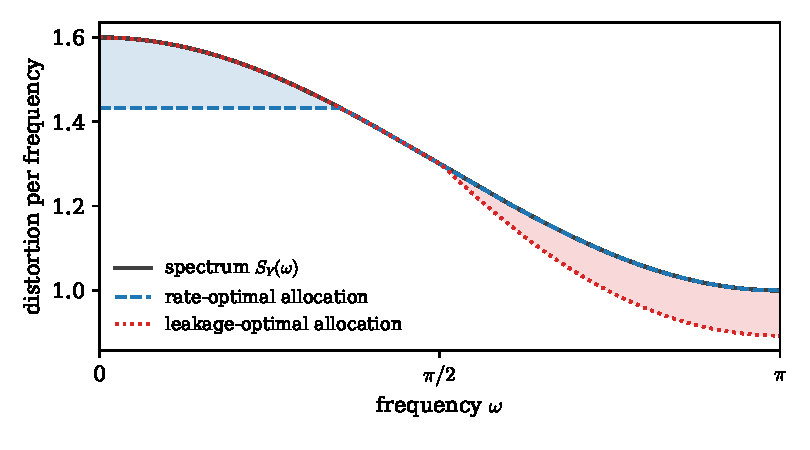
\includegraphics[width=0.72\linewidth]{fig_bands.pdf}
\caption{Distortion allocations of the rate-optimal and the
leakage-optimal descriptions for the disjoint-bands instance, with the
spectrum $S_Y$. A frequency is described where the allocation lies
below $S_Y$. The two descriptions describe disjoint bands.}
\label{fig:bands}
\end{figure}

\emph{Convergence in the period.} For a random two-dimensional source
with a three-tap moving-average spectrum, a scalar described variable,
and a scalar holder with a two-tap filter, at $D=0.4D_{\max}$, the
weighted cost of the period-$n$ source differs from the spectral value
by $1.8\times10^{-3}$, $1.3\times10^{-6}$, and $1.7\times10^{-8}$ bits at $n=8$, $32$, and $128$, at $\alpha=0$
(Table~\ref{tab:conv}).

\emph{Windows.} For the pair of Section~\ref{sec:retention} with
$\rho=0.8$, $a=0.7$, $\tau^2=0.5$, and $D=0.5$, the window cost at
$\alpha=0$ exceeds the spectral value by $1.59\times10^{-2}$, $3.98\times10^{-3}$, and $1.99\times10^{-3}$ bits at $N=8$,
$32$, and $64$, and $N$ times the gap is $0.127$ at each
(Table~\ref{tab:conv}). For a spectrum outside the affine class the gap
at $\alpha=0$ is $3.18\times10^{-3}$, $7.7\times10^{-4}$, and $5.1\times10^{-4}$ bits at $N=8$, $32$, and $48$, and
$N$ times the gap settles near $0.025$. In every case computed the window
cost lies above the spectral value and the gap decays like $1/N$. This
is evidence for Conjecture~\ref{conj:windows} and not a proof.

\begin{table}[t]
\centering
\caption{Distance from the spectral value, in bits per symbol. Left:
the source of period $n$ (Theorem~\ref{thm:spectral}). Right: windows of
the stationary source, for an affine spectrum
(Theorem~\ref{thm:affine}) and a general one
(Conjecture~\ref{conj:windows}). The periodic source converges fast, the
windows like $1/N$ from above.}
\label{tab:conv}
\begin{tabular}{rccc@{\qquad}rcc@{\qquad}rcc}
\hline
 & \multicolumn{3}{c}{period $n$, $|V_n-V|$} & & \multicolumn{2}{c}{affine, $V^{\mathrm w}_N-V$} & & \multicolumn{2}{c}{general, $V^{\mathrm w}_N-V$}\\
$n$ & $\alpha=0$ & $\alpha=0.5$ & $\alpha=1$ & $N$ & $\alpha=0$ & $\alpha=0.5$ & $N$ & $\alpha=0$ & $\alpha=1$\\
\hline
8 & $1.8\times10^{-3}$ & $1.1\times10^{-3}$ & $1.8\times10^{-3}$ & 8 & $1.59\times10^{-2}$ & $2.08\times10^{-2}$ & 8 & $3.18\times10^{-3}$ & $1.65\times10^{-2}$\\
32 & $1.3\times10^{-6}$ & $1.4\times10^{-5}$ & $2.2\times10^{-5}$ & 16 & $7.96\times10^{-3}$ & $1.04\times10^{-2}$ & 16 & $1.56\times10^{-3}$ & $8.17\times10^{-3}$\\
128 & $1.7\times10^{-8}$ & $2.5\times10^{-7}$ & $6.3\times10^{-7}$ & 32 & $3.98\times10^{-3}$ & $5.19\times10^{-3}$ & 32 & $7.7\times10^{-4}$ & $4.07\times10^{-3}$\\
512 & $8\times10^{-11}$ & $5.5\times10^{-9}$ & $1.4\times10^{-8}$ & 64 & $1.99\times10^{-3}$ & $2.59\times10^{-3}$ & 48 & $5.1\times10^{-4}$ & $2.71\times10^{-3}$\\
\hline
\end{tabular}
\end{table}

\emph{What the holder keeps.} For the same pair and $D=0.4$, the
conditional variances are $q=0.9216$ for one sample at lag $3$,
$0.2823$ for the causal prefix with no wait, $0.24484$ for the causal
prefix with a wait of three symbols, and $0.24481$ for the whole path,
with $P_f=0.2823$ and $C=0.3048$. The least leakages are $0.6386$,
$0.3769$, $0.3524$, and $0.3524$ bits, against a rate of $0.6610$ bits.
A holder that kept one stale sample gains almost nothing from it, since
the description conveys to it nearly its whole rate. A holder that kept
its past is conveyed a little over half the rate, and three symbols of
waiting bring it to within $10^{-4}$ bits of the holder that keeps
everything.

\section{Discussion}
\label{sec:discussion}

What is established has four scopes, and they should be kept apart.
For independent blocks with circulant covariance the region is exact
and operational (Theorem~\ref{thm:periodic}). The spectral program is
the exact limit of those regions (Theorem~\ref{thm:spectral}). For the
stationary source with a spectrum affine in one scalar spectrum and a
memoryless holder, the spectral region is the operational region, with
a converse through windows and a coding theorem with a randomized
encoder (Theorems~\ref{thm:affine} and~\ref{thm:achieve}). For a general
stationary source the converse through windows holds
(Proposition~\ref{prop:window}), convergence of the windows is
conjectured, and achievability follows from that convergence for
trigonometric polynomial spectra. Within those scopes, the
frontier of rate and leakage is reverse water-filling on a tilted
weight at each frequency, under one level. The level is the only thing
the frequencies share. Which
frequencies a description occupies is decided by the spectrum for the
decoder and by the spectrum times a coherence factor for the holder,
and the two can disagree completely. A delay in the holder's
observation is free of consequence when the holder has its whole
observation, and for a one-symbol description the cost of staleness is
the cost of holding less of it.

The allocation over frequencies, the activation order, and the
possibility of disjoint supports are those of independent components in
\cite[Theorem~27, Corollary~28]{part1}, with frequencies in the place of
components. What this paper adds to \cite{part1} is the passage to
sources with memory: the exact splitting for periodic sources with
arbitrary matrix geometry within each frequency, the spectral limit
with a level that moves with the period, the window results and the
coding theorem for the stationary source in the affine class, and the
reduction of what the holder keeps to one variance. The coding theorem
covers the affine class with a memoryless holder and a randomized
encoder. Beyond that class it is conditional on the convergence of the
windows.

Several problems are open. The convergence of the window regions to
the spectral region is proved for affine spectra and conjectured in
general, and with it the operational region outside the affine class.
Whether the randomization at the encoder can be removed is open. The holder that keeps a causal prefix is treated for
one-symbol descriptions only, and block codes against such a holder are
open, as is the decoder with a delay constraint. Side information at
the decoder, which \cite{part1} leaves partly open for memoryless
sources, is not treated. Finite blocklengths and non-Gaussian processes
are not treated.

\appendices

\section{Numerical Checks and Formal Verification}
\label{app:numver}
\sloppy

The statements were checked independently of the derivations. The
scripts, their recorded outputs, and a notebook that reruns them are in
the public repository
\texttt{https://github.com/ahb-sjsu/geometric-observation}, directory
\texttt{paper/tit-stationary}. No proof depends on them.

\texttt{spectral\_core.py} implements the costs and one solver, the
water-filling iteration of \cite[Proposition~11]{part1} with a bisection
on the level. The solver uses no structure of its input, so the same
code solves a window problem as one real matrix program and the
per-frequency Hermitian programs. \texttt{verify\_spectral.py} runs nine
checks with a fixed seed. For Theorem~\ref{thm:periodic} it solves the
period-$n$ problem in $\R^{pn}$ with no structure assumed, on $48$
instances with $p$ up to four and holders of rank up to three, and
compares it with the per-frequency solution: the costs agree to
$9\times10^{-14}$ bits, the solutions to $3\times10^{-12}$, the
unstructured solution is block-diagonal in the Fourier basis to
$2\times10^{-15}$, and the assembled spectral solution satisfies the
optimality condition of \cite[Theorem~7]{part1} in the full space to
$3\times10^{-13}$. It checks the convergence of
Theorem~\ref{thm:spectral}, the reduction to Kolmogorov's formula
($10^{-12}$ bits), the closed form, the allocation, and the activation
rule of Theorem~\ref{thm:pair} on a pair with a complex
frequency-dependent cross-spectrum ($2\times10^{-15}$ bits, $3\times10^{-13}$,
and no frequency misclassified), the instance of
Corollary~\ref{cor:bands}, Proposition~\ref{prop:allpass} for delays of
zero to four symbols in the full real space, the exact splitting and
the convergence of Theorem~\ref{thm:affine}, the computed gaps for
Conjecture~\ref{conj:windows}, and Proposition~\ref{prop:retention}
against a direct solution with the retained observations as a vector
holder. The output is recorded in
\texttt{verify\_spectral-2026-11-13.txt}. \texttt{sweep\_bands.py}
computes Table~\ref{tab:sweep} and the budget at which the supports
first overlap, recorded in \texttt{sweep\_bands-2026-11-13.txt}.
\texttt{verify\_achievability.py} checks the steps of the proof of
Theorem~\ref{thm:achieve} that are statements about covariances, in both
cases of the decomposition: the decomposition itself, the independence
of blocks separated by guard intervals, the coupling, and the two
leakage inequalities on Gaussian stand-ins for the message. The
perturbation bound is loose at the sizes computed, where the measured
change in leakage is $0.03$ bits against a bound of several bits, and
only its vanishing with the remainder's power is used. The coding
theorem itself is not something a computation verifies. The output is
recorded in \texttt{verify\_achievability-2026-11-13.txt}.
\texttt{reproduce.ipynb} reruns the checks, shows the sweep, and draws
the figure. A reviewer of a draft recomputed the instance at
$D=0.97D_{\max}$ independently, including a direct optimization over the
scalar error covariance, and obtained the same rates, leakages, and
supports.

The Lean~4 module
\texttt{lean/ObservationTheory/SpectralRateLeakage.lean} (Mathlib,
twenty-one theorems, no \texttt{sorry}, only the standard axioms)
machine-checks the algebraic steps: for the per-direction costs
$\tfrac12\ln(1/x)$ and $\tfrac12\ln((1+jx)/(x(1+j)))$, that the leakage
is nonnegative, at most the rate, and nonincreasing in the holder's
information $j$; the slope of the weighted cost and its equivalence
with the quadratic of Section~\ref{sec:spectral}; that the quadratic
has exactly one positive root; the activation threshold; the optimality
of a common-slope allocation in its finite form and in the integral
form used in Lemma~\ref{lem:limit}(b); the invariance of
$H^{\herm}MH$ under a unit-modulus factor
(Proposition~\ref{prop:allpass}); that a real block matrix commuting
with $\mathsf J$ is the image under $\varrho$ of a complex matrix, and
conversely (Lemma~\ref{lem:hermitian}); that invariance under a sign
symmetry forces a block-diagonal form; and that matrices affine in one
matrix commute (Theorem~\ref{thm:affine}). Not formalized are
Lemma~\ref{lem:limit}(a) and (c), the determinant and spectral
properties of $\varrho$, the block-circulant step of
Theorem~\ref{thm:periodic}, Szeg\H{o}'s theorem, the proof of
Theorem~\ref{thm:achieve}, and everything imported from \cite{part1}. The build and the axiom audit are recorded
in \texttt{lean-spectral-2026-11-13.txt}.

\section*{Acknowledgment}

In accordance with the IEEE policy on AI-generated text, the author
discloses the use of Anthropic's Claude models (Claude Fable 5.2)
through the Claude Code environment in 2026, for drafting prose and
proofs from the author's statements of the results, for the prior-art
search, for the check scripts and the Lean module, and for independent
passes on the proofs. The author is responsible for the content.

\begin{thebibliography}{99}
\bibitem{part1} A. H. Bond, ``Rate, leakage, and distortion for Gaussian
sources: Water-filling on a tilted weight,'' submitted to \emph{IEEE
Trans. Inf. Theory}, 2026, archived at
\url{https://doi.org/10.5281/zenodo.23127802}.
\bibitem{kolmogorov1956} A. N. Kolmogorov, ``On the Shannon theory of
information transmission in the case of continuous signals,'' \emph{IRE
Trans. Inf. Theory}, vol. 2, no. 4, pp. 102--108, 1956.
\bibitem{berger1971} T. Berger, \emph{Rate Distortion Theory: A Mathematical
Basis for Data Compression}. Englewood Cliffs, NJ: Prentice-Hall, 1971.
\bibitem{villard2013} J. Villard and P. Piantanida, ``Secure multiterminal
source coding with side information at the eavesdropper,'' \emph{IEEE
Trans. Inf. Theory}, vol. 59, no. 6, pp. 3668--3692, 2013.
\bibitem{ekrem2013} E. Ekrem and S. Ulukus, ``Secure lossy transmission of
vector Gaussian sources,'' \emph{IEEE Trans. Inf. Theory}, vol. 59, no. 9,
pp. 5466--5487, 2013.
\bibitem{xu2024} Y. Xu, G. Chen, J. Chen, and S. Jin, ``New proofs of
Gaussian extremal inequalities with applications,'' \emph{IEEE Trans.
Inf. Theory}, vol. 70, no. 5, pp. 3082--3099, May 2024.
\bibitem{sankar2011} S. R. Rajagopalan, L. Sankar, S. Mohajer, and
H. V. Poor, ``Smart meter privacy: A utility-privacy framework,'' in
\emph{Proc. IEEE Int. Conf. Smart Grid Commun. (SmartGridComm)}, 2011,
pp. 190--195, arXiv:1108.2234.
% verify authors' order, title, and pages on final (arXiv record confirms the venue and DOI 10.1109/SmartGridComm.2011.6102315 only).
\bibitem{sankar2013} L. Sankar, S. R. Rajagopalan, S. Mohajer, and
H. V. Poor, ``Smart meter privacy: A theoretical framework,'' \emph{IEEE
Trans. Smart Grid}, vol. 4, no. 2, pp. 837--846, 2013.
% verify on final: the journal text was not read.
\bibitem{liu2016} J. Liu, P. Cuff, and S. Verd\'u, ``Key capacity for
product sources with application to stationary Gaussian processes,''
\emph{IEEE Trans. Inf. Theory}, vol. 62, no. 2, pp. 984--1005, 2016.
\bibitem{dikshtein2022} M. Dikshtein, N. Weinberger, and S. Shamai, ``On
information bottleneck for Gaussian processes,'' in \emph{Proc. IEEE Inf.
Theory Workshop (ITW)}, 2022, pp. 546--551.
\bibitem{gray1973} R. M. Gray, ``A new class of lower bounds to information
rates of stationary sources via conditional rate-distortion functions,''
\emph{IEEE Trans. Inf. Theory}, vol. 19, no. 4, pp. 480--489, 1973.
\bibitem{leiner1974} B. M. Leiner and R. M. Gray, ``Rate-distortion theory
for ergodic sources with side information (Corresp.),'' \emph{IEEE Trans.
Inf. Theory}, vol. 20, no. 5, pp. 672--675, 1974.
\bibitem{dobrushin1962} R. L. Dobrushin and B. S. Tsybakov, ``Information
transmission with additional noise,'' \emph{IRE Trans. Inf. Theory},
vol. 8, no. 5, pp. 293--304, 1962.
\bibitem{simeone2013} O. Simeone and H. H. Permuter, ``Source coding when
the side information may be delayed,'' \emph{IEEE Trans. Inf. Theory},
vol. 59, no. 6, pp. 3607--3618, 2013.
\bibitem{pearl1973} J. Pearl, ``On coding and filtering stationary signals
by discrete Fourier transforms,'' \emph{IEEE Trans. Inf. Theory}, vol. 19,
no. 2, pp. 229--232, 1973.
% verify vol/pages on final
\bibitem{gray2006} R. M. Gray, ``Toeplitz and circulant matrices: A
review,'' \emph{Found. Trends Commun. Inf. Theory}, vol. 2, no. 3,
pp. 155--239, 2006.
\bibitem{grenander1958} U. Grenander and G. Szeg\H{o}, \emph{Toeplitz Forms
and Their Applications}. Berkeley, CA: Univ. California Press, 1958.
\bibitem{gutierrez2012} J. Guti\'errez-Guti\'errez and P. M. Crespo, ``Block
Toeplitz matrices: Asymptotic results and applications,'' \emph{Found.
Trends Commun. Inf. Theory}, vol. 8, no. 3, pp. 179--257, 2012.
% verify year on final: Crossref gives 2012, the publisher's suggested citation 2011.
\bibitem{berge1963} C. Berge, \emph{Topological Spaces}, transl.
E. M. Patterson. Edinburgh, U.K.: Oliver and Boyd, 1963.
\bibitem{rockafellar1970} R. T. Rockafellar, \emph{Convex Analysis}.
Princeton, NJ: Princeton Univ. Press, 1970.
\bibitem{rts1965} H. E. Rauch, F. Tung, and C. T. Striebel, ``Maximum
likelihood estimates of linear dynamic systems,'' \emph{AIAA J.}, vol. 3,
no. 8, pp. 1445--1450, 1965.
% verify vol/pages on final
\end{thebibliography}

\end{document}
